%%%%%%%%%%%%%%%%%%%%%%%%%%%%%%%%%%%%%%%%%%%%%%%%%%%%%%%%%%%%%%%%%%%%%%
%%%%                   Submap
%%%%%%%%%%%%%%%%%%%%%%%%%%%%%%%%%%%%%%%%%%%%%%%%%%%%%%%%%%%%%%%%%%%%%%

\color{red}

A \glyph{submap} is used to encapsulate entities and relationships (including all types of nodes and edges) within one named glyph. The content of the submap can be found for instance on another (web) page in the case of static maps, or can be displayed dynamicaly. Because of the independence of rules, no particular connections are needed between the submap and the containing map.

\begin{figure}[H]
  \centering
  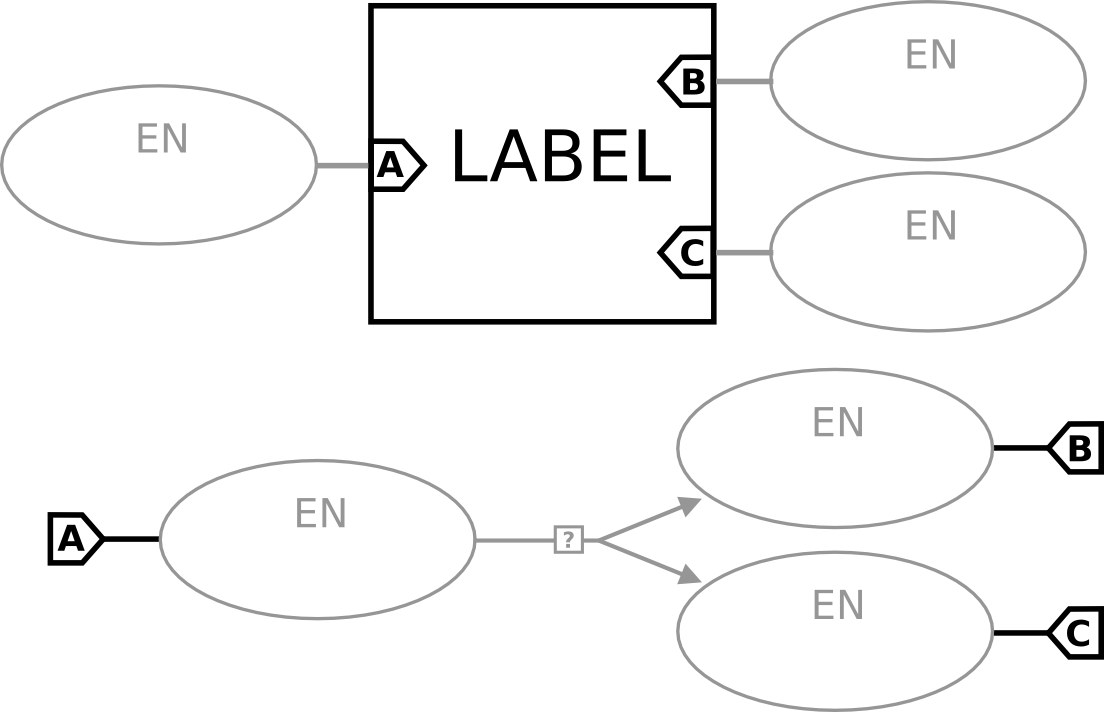
\includegraphics[scale = 0.3]{images/submap}
  \caption{The \ER glyph for \glyph{submap}.}
  \label{fig:submap}
\end{figure}


\normalcolor
